
\chapter{Metodologias e Mecanismos de Participação Implementados}
\label{Att:ferramentasparticipacao}

Como visto na imagem ilustrada pela figura \ref{fig:arquiteturaparticipa}, o Participa.br já adotou várias das ferramentas de participação propostas na figura, algumas delas já vem como padrão no framework utilizado para o desenvolvimento (Noosfero). Outras ferramentas foram desenvolvidas e acopladas na ferramenta, pois utilizam metodologias específicas, como é o caso do PairWise, que utiliza a metodologia do All Our Ideas. Neste anexo é apresentado as principais ferramentas desenvolvidas pelos consultores do Participa.br.

\section*{Agenda de Eventos}

Essa ferramenta é composta por uma agenda, que contém todos os eventos relacionados a participação social. Esses eventos podem ser presenciais ou mesmos a distância, utilizando outras ferramentas de apoio, como a transmissão de eventos ao vivo. Os usuários também podem criar seus próprios eventos, divulgando o mesmo em redes sociais ou no próprio Participa.br.

\section*{Blog}

Espaço onde os usuários podem postar suas opiniões em forma de post ou artigos, com suporte à mídias como áudios, vídeos e imagens. O blog é um espaço livre dentro do perfil de cada usuário, onde o mesmo é responsável por controlar os assuntos postados, frequência, controle dos comentários escritos por outros usuário, entre outros.

\section*{Comunidades Temáticas}

São comunidades dentro da plataforma Participa.br, que possuem um grupo de interessados no mesmo assunto. Essas comunidades possuem temas sobre determinados assuntos, que tem como objetivo se tornar um espaço para a formulação e debate de ideias que no final devem se tornar políticas públicas.

%

As comunidades temáticas são geridas por representantes do Governo e da Sociedade Civil. Como dito anteriormente, nas comunidades temáticas só é possível o usuário participar da mesma se o mesmo estiver cadastrado. Depois de participar da mesma, o usuário pode participar e/ou contribuir nas ferramentas de participação que aquela comunidade disponibiliza.

\graphicspath{{figuras/}}
\begin{figure}[H]
\centering
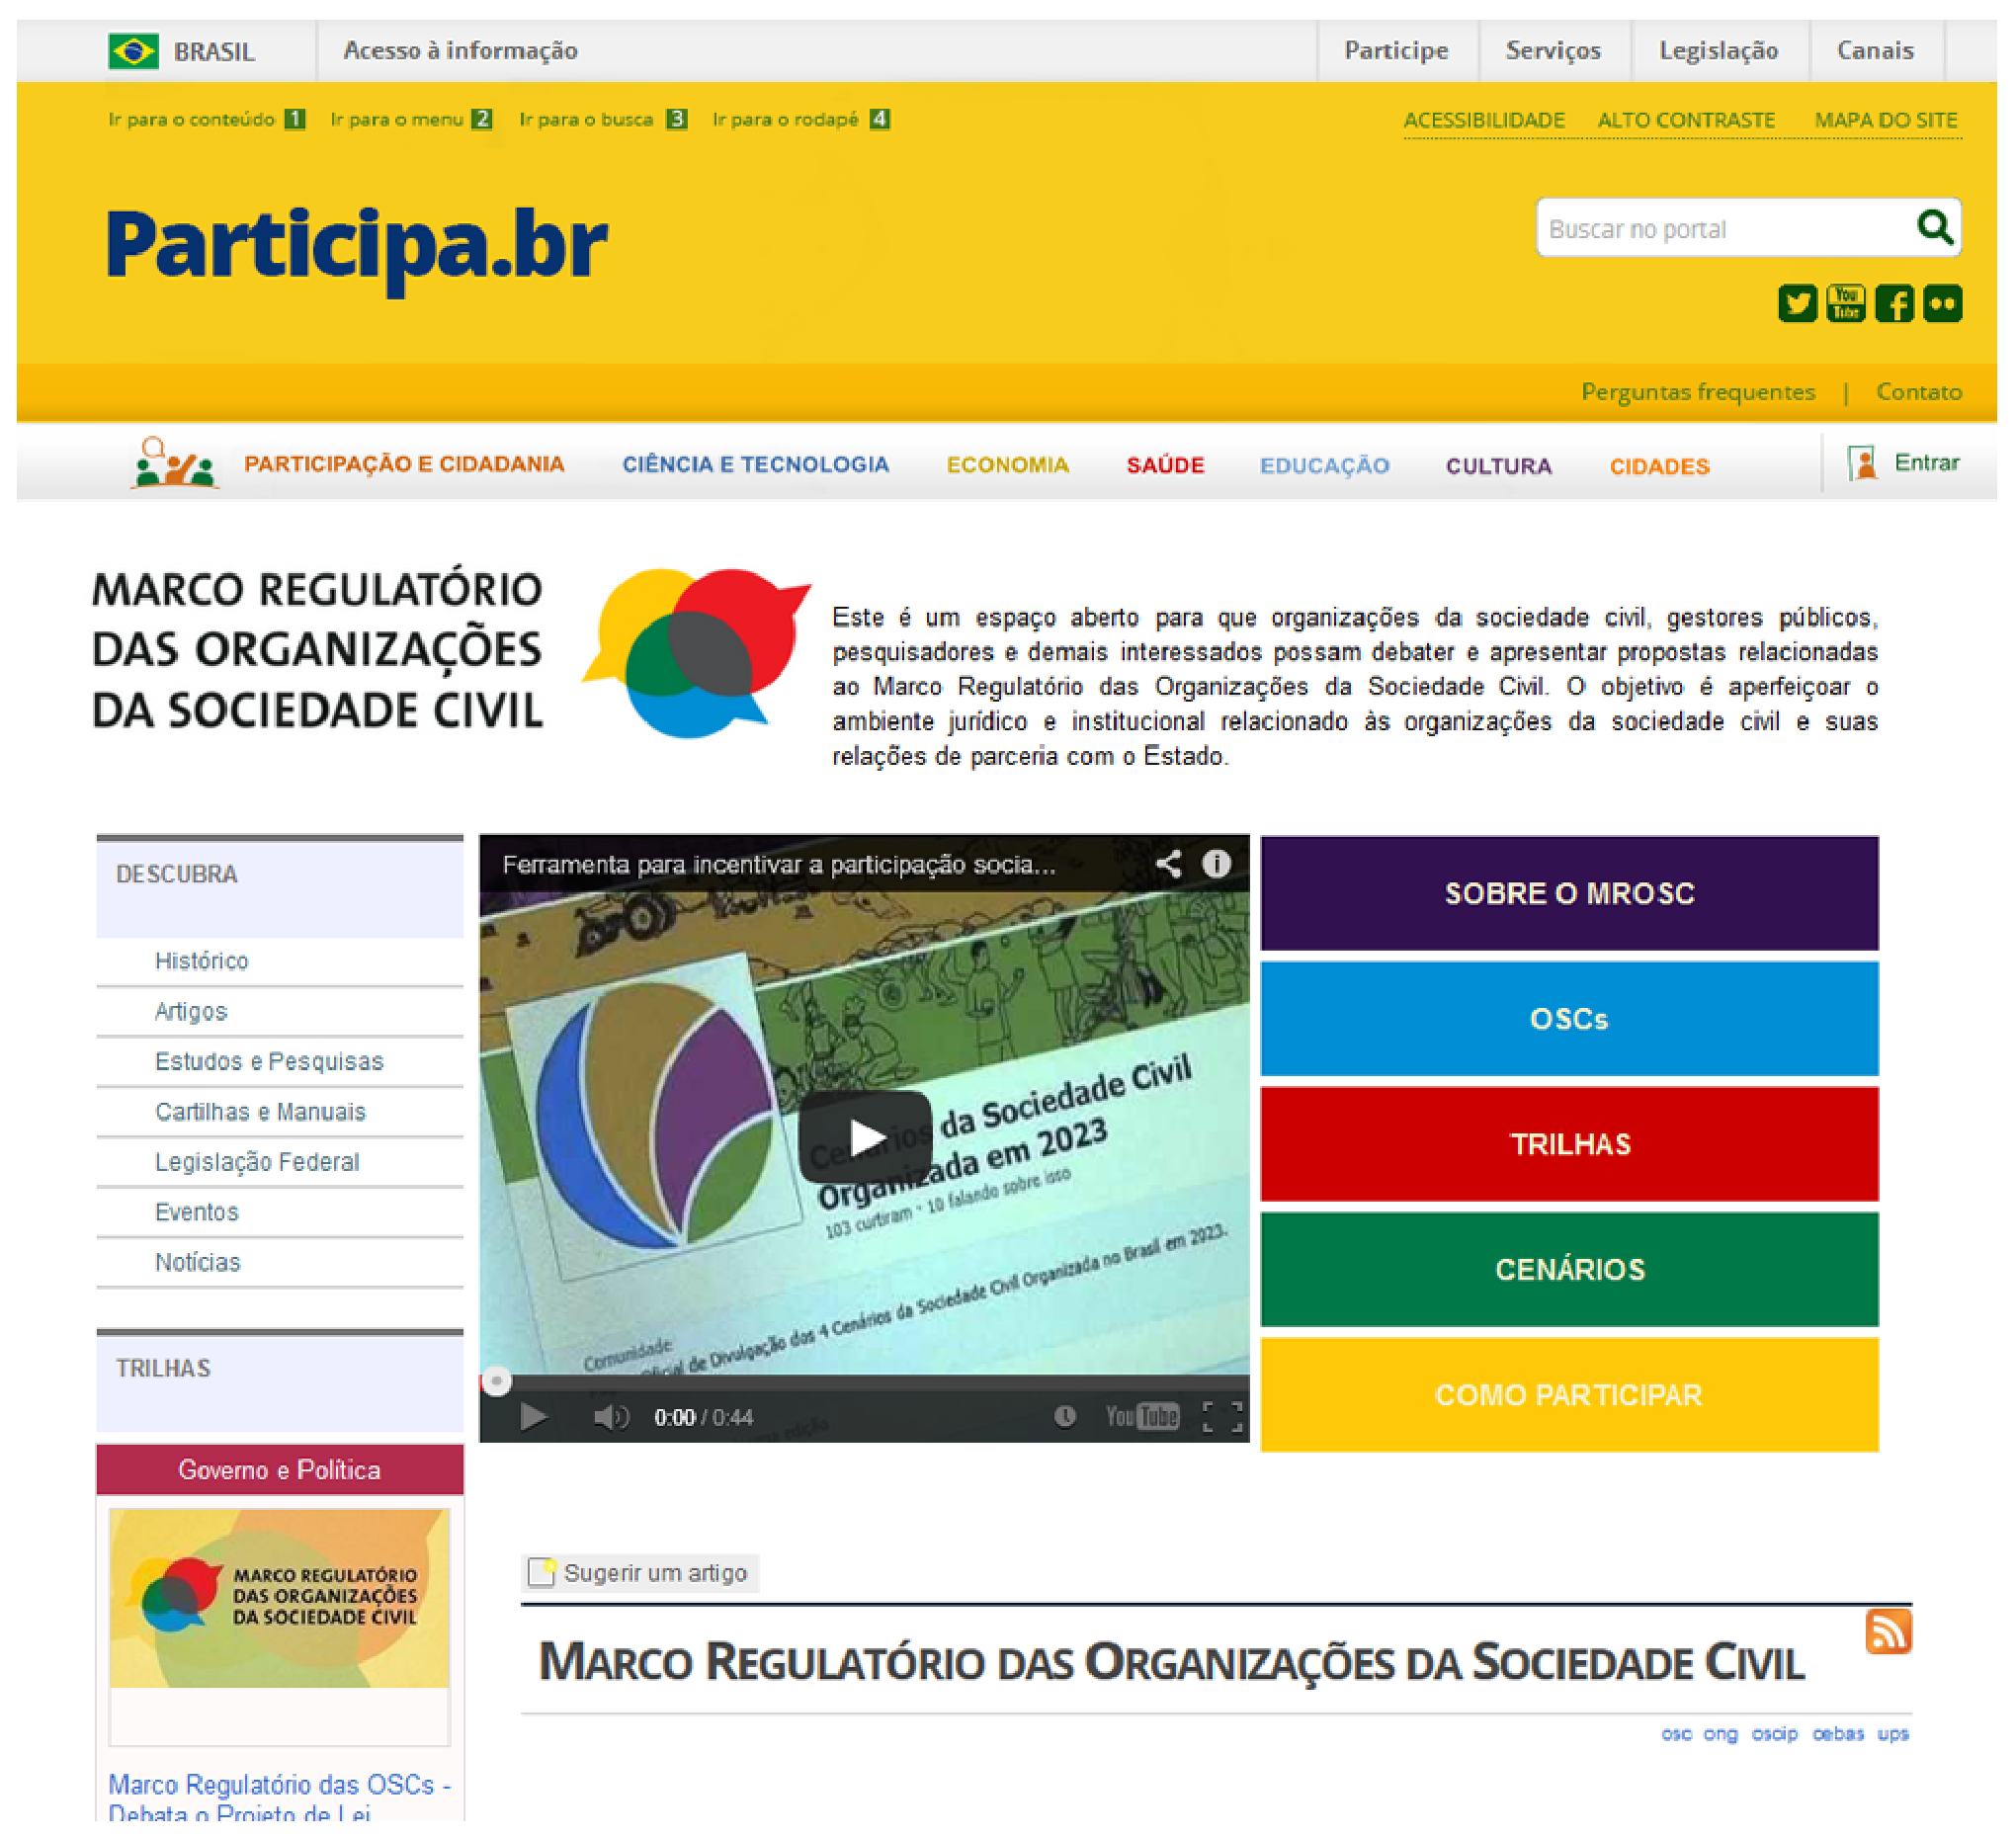
\includegraphics[width=0.7\textwidth]{comunidades-tematicas}
\caption{Comunidade Temática.}
\label{fig:comunidadestematicas}
\end{figure}


\section*{Comentário por Parágrafo}

Nessa ferramenta, o administrador de conteúdo disponibiliza um artigo de texto, onde são escolhido alguns trechos do mesmo. A cada pedaço desse texto é criado um local para comentários, onde participante pode opinar dentro daquele trecho, dando sugestões e/ou propostas para debater sua idéia e sugerir melhorias para o texto.

\graphicspath{{figuras/}}
\begin{figure}[H]
\centering
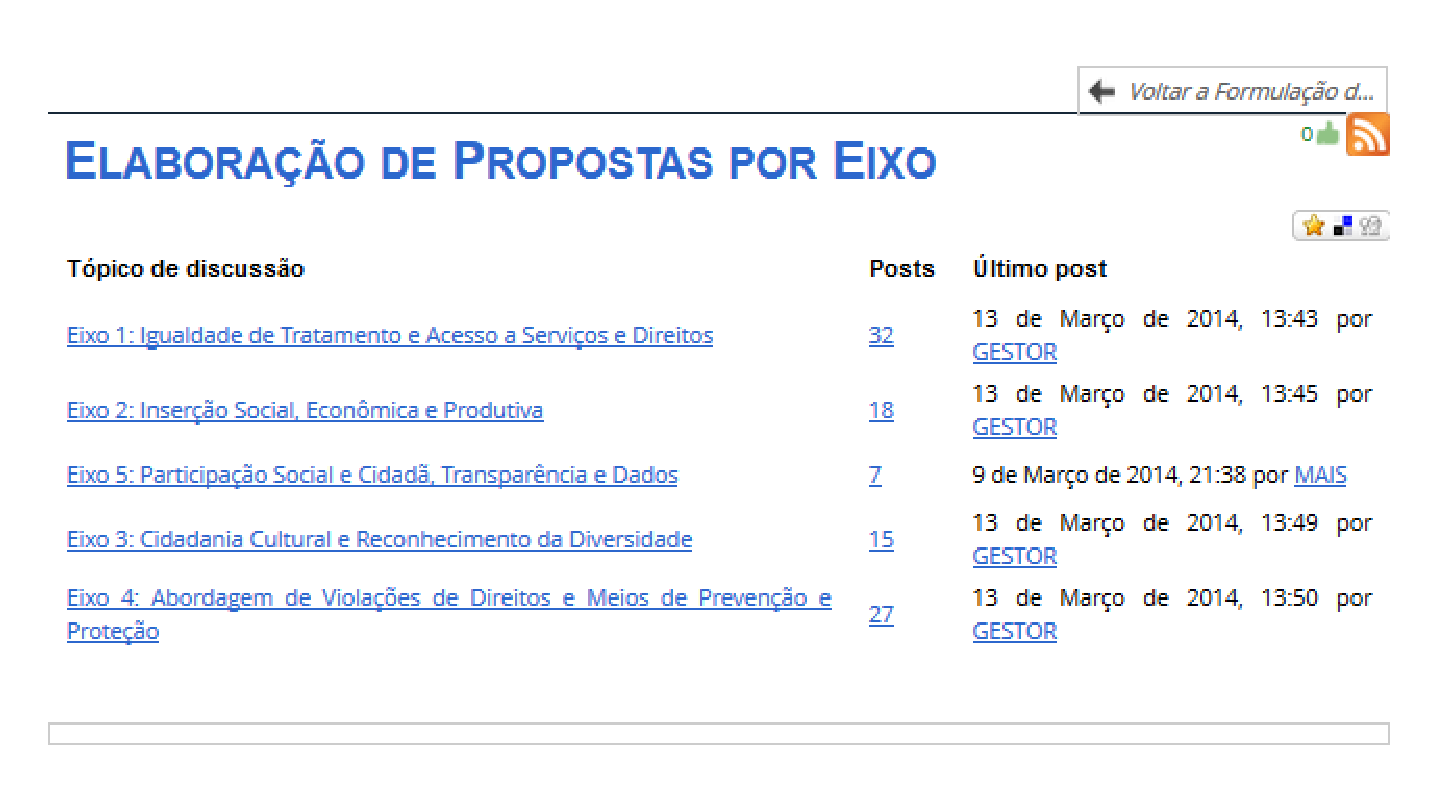
\includegraphics[width=0.7\textwidth]{foruns-participacao}
\caption{Fórum de Participação.}
\label{fig:forumsparticipacao}
\end{figure}


\section*{Fóruns de Discussão}

A ferramenta fórum de discussão é semelhante em questões de funcionamento, a outros fóruns de discussão encontrados pela internet. Nessa ferramenta é escolhida uma questão e postado através de um tópico e os usuários podem debater sobre aquele tema através de posts. No final o resultado de cada tópico, pode se tornar insumos para elaboração de alguma política pública.

\graphicspath{{figuras/}}
\begin{figure}[H]
\centering
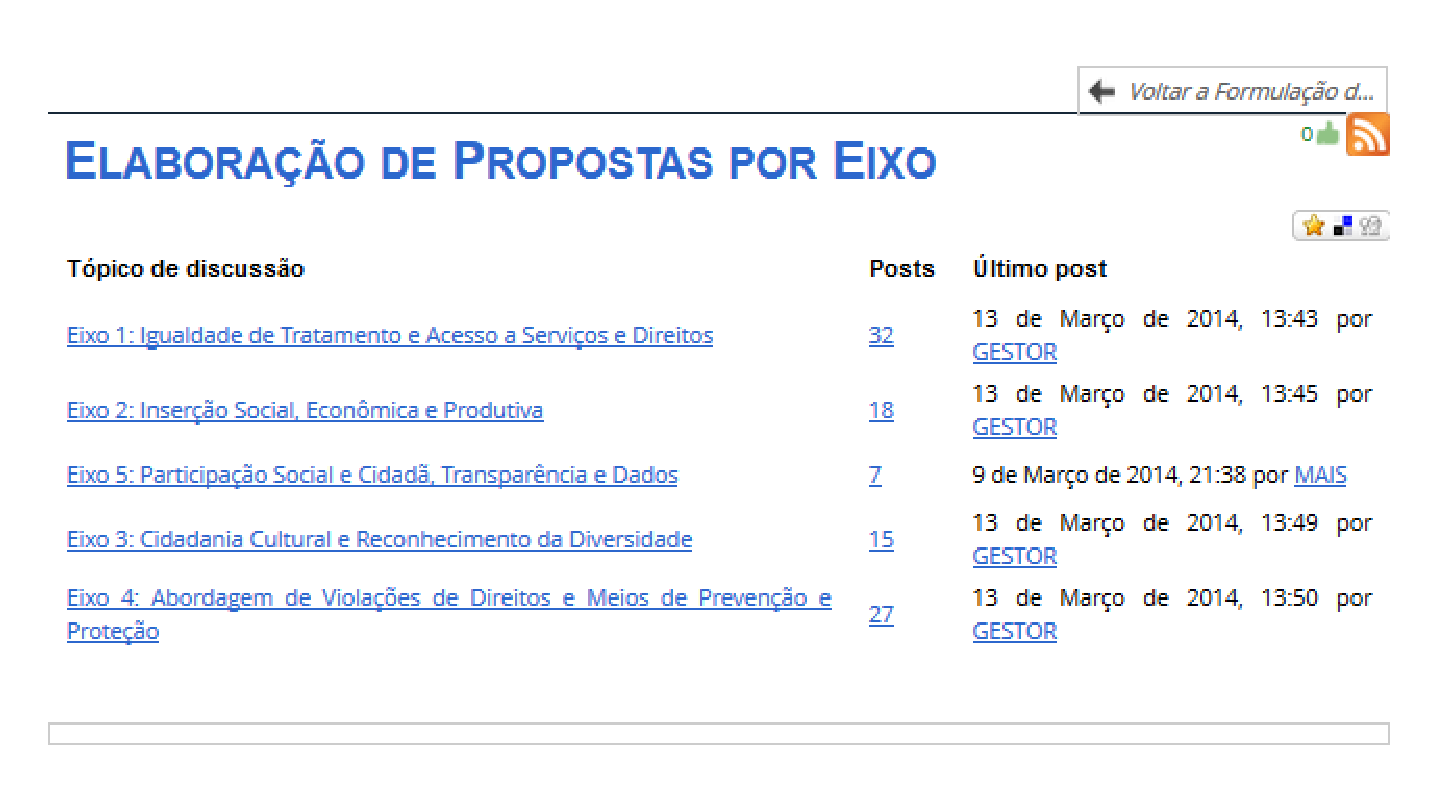
\includegraphics[width=0.7\textwidth]{foruns-participacao}
\caption{Fórum de Participação.}
\label{fig:forumsparticipacao}
\end{figure}

\section*{Hub}

O Hub é uma ferramenta que permite a interação ao-vivo entre os participantes. Através de um chat, as pessoas podem acompanhar a transmissão discutindo um determinado assunto. Também há um chat moderado, onde as pessoas discutem sobre um assunto que é colocado em pauta. 

\section*{Realização de Conferências Virtuais}

Nas conferências virtuais, os participantes participam através do conjunto de ferramentas e mecanismos de participação que Participa.br fornece. Essas ferramentas ajudam as conferências na utilização da plataforma para realização de etapas online.

A primeira Conferência que utilizou a plataforma Participa.br como plataforma escolhida foi a COMIGRAR\footnote{\url{http://www.participa.br/comigrar}} (Conferência Nacional sobre Migrantes e Refúgio).

\section*{Realização de Consultas Públicas e Priorização de Ideias (Pairwise)}

Nessa ferramenta os usuários participam de uma votação para definição sobre a um tema determinado. O participante responde várias perguntas definidas pelos administradores de conteúdo, cada uma com um par de propostas, sem limites de respostas. A cada pergunta o usuário votava na opção que se concordava mais, caso não houvesse nenhuma proposta que ele mais se identificasse ele poderia sugerir novas propostas.

Solagna (\citeyear{solagna2014metodologias}) diz que a aplicação do PairWise durante 2 anos Gabinete Digital do Rio Grande do Sul demonstrou que a metodologia tem potencial para grandes consultas e grandes votações. A utilização desta ferramenta como forma de priorização de ideias é a melhor alternativa para evitar problemas metodológicos com desvios a partir de grupos de interesse.

\section*{Transmissão Online de Eventos Presenciais}

As transmissões online é a disponibilização de um evento ao vivo na plataforma Participa.br através de streaming de áudio e vídeo. Juntamente com o streaming, existe um chat onde os visualizadores daquele evento podem interagir com os outros participantes através da utilização de outras redes sociais utilizando hashtags.

\section*{Trilhas de Participação}

A Trilha de Participação é um local para a debates de idéias e troca de experiência colaborativa, para construção de políticas públicas. Uma triha é a forma de como um tema é debatido dentro de uma comunidade, desde a criação da comunidade até a criação de uma determinada política pública.

A Trilha de Participacação funciona através de etapas, onde cada etapa possui um mecanismo de participação (forúns, consulta pública, comentários por paragráfo, pairwise, entre outros), que é escolhido pelo administrador. 
